\documentclass[12pt,a4paper,titlepage,oneside]{book}

% --------------------------------------------------
% Page layout
% --------------------------------------------------
\usepackage[
    a4paper,
    hdivide={28mm,*,22mm},
    vdivide={25mm,*,20mm},
    nofoot
]{geometry}

% --------------------------------------------------
% Fonts / typography
% --------------------------------------------------
\usepackage[utf8]{inputenc}
% \usepackage{microtype}
\usepackage{setspace}
\onehalfspacing
\frenchspacing

% Optional: uncomment if you want slightly more spacious
% thesis-style line spacing
% \onehalfspacing

% --------------------------------------------------
% Mathematics
% --------------------------------------------------
\usepackage{amsmath,amssymb}

% --------------------------------------------------
% Figures / tables
% --------------------------------------------------
\usepackage{graphicx}
\usepackage{booktabs}
\usepackage[bf]{caption}

% --------------------------------------------------
% Diagrams
% --------------------------------------------------
\usepackage{tikz}
\usetikzlibrary{arrows.meta,positioning,fit,backgrounds}

% --------------------------------------------------
% Floating figures/tables
% --------------------------------------------------
\usepackage{float}

% --------------------------------------------------
% Hyperlinks
% --------------------------------------------------
\usepackage[hidelinks]{hyperref}

% --------------------------------------------------
% Bibliography
% --------------------------------------------------
\usepackage[numbers,sort&compress]{natbib}

\bibliographystyle{IEEEtran}

% --------------------------------------------------
% Chapter formatting
% --------------------------------------------------
\usepackage{titlesec}

\titleformat{\chapter}[hang]
    {\normalfont\huge\bfseries}
    {\thechapter}
    {1em}
    {}

% --------------------------------------------------
% Document naming
% --------------------------------------------------
\renewcommand{\bibname}{References}

\begin{document}

\begin{titlepage}
\centering
\vspace*{\fill}
{\huge Johannes Kepler University Linz\par}
\vspace{1cm}
{\Large Bachelor's Thesis\par}
\vspace{4.0cm}

{\Huge \textbf{ArxivRAG: Retrieval-Augmented Generation for Scientific Literature}\par}
\vspace{4.0cm}

\begin{center}
\large
\begin{tabular}{@{}l l@{}}
\textbf{Author:} & Raymond Denis Vladu (K1230746) \\
\textbf{Program:} & BSc Artificial Intelligence \\
\textbf{Supervisor:} & Lukas Hauzenberger \\
\textbf{Date:} & \today \\
\end{tabular}
\end{center}
\vspace*{\fill}
\end{titlepage}

\chapter*{Abstract}
Large language models generate fluent text but store knowledge in parameters that are hard to update and prone to hallucination, a limitation that is especially acute for scientific question answering, where factual grounding and source attribution are essential. Retrieval-Augmented Generation (RAG) addresses this by pairing a parametric generator with a non-parametric external memory accessed through retrieval. This thesis consolidates RAG theory with the design and evaluation of \textit{ArxivRAG}, a retrieval-augmented system for question answering over arXiv papers, unifying a seminar literature review and a practical implementation project.

The documented pipeline searches and downloads arXiv papers, parses and chunks their content, embeds and indexes the chunks, and serves queries through dense or hybrid retrieval with optional cross-encoder reranking before grounded generation. The same pipeline is exposed through an interactive web application that fetches papers live, indexes them ephemerally, generates answers for all four chunking strategies, and surfaces cited sources. Retrieval quality is assessed on a manually curated benchmark of 49 questions over frozen corpus snapshots, using rank-aware metrics (Hit@k, Coverage@k, Precision@k, MRR, and MAP) with 95\% bootstrap confidence intervals and paired significance tests. Experiments compare chunking, retrieval mode, top-$k$, reranking, and embedding models, with relevance scored by a fixed judge embedder held constant across runs.

Chunking is the dominant design variable: the gap between the best and worst strategy far exceeds the effect of retrieval mode, reranking, or embedding model. Fixed-window chunking with dense retrieval at top-$k=10$ and no reranking is the strongest all-round operating point; reranking improves precision at small $k$ at the cost of coverage. Given the benchmark size, several configurations remain statistically indistinguishable. The interactive application operationalizes the topics-and-query workflow but still serves all four chunkers as a qualitative comparison tool rather than locking to this configuration. The thesis evaluates the retrieval stage only; scoring generated-answer quality is left as future work.
\clearpage

\tableofcontents
\clearpage

\listoftables
\clearpage

\listoffigures
\clearpage

\chapter{Introduction}

This thesis studies Retrieval-Augmented Generation (RAG) for scientific literature, with a focus on arXiv papers. The work builds on two prior course projects: a seminar literature review on RAG and a practical implementation project (\textit{ArxivRAG}) that designed a retrieval pipeline, an interactive web application, and a retrieval benchmark.

Large language models provide fluent generation but store knowledge in model parameters that are difficult to update and may produce hallucinations. RAG addresses this by combining a parametric generator with non-parametric external memory accessed through retrieval \cite{lewis2020rag}. This hybrid design is especially relevant for scientific domains, where factual grounding and source-aware responses are critical.

The practical project showed that retrieval quality in scientific corpora depends strongly on engineering decisions such as chunking strategy, retrieval mode, top-$k$, and reranking. Using a frozen evaluation corpus and a manually curated benchmark set, the best tested configuration was fixed-window chunking with dense retrieval at top-$k=10$ and reranking disabled. In parallel, the same codebase ships a working interactive application that lets a user enter topics and a question, fetches matching arXiv papers, and returns grounded answers with cited sources.

The goal of this thesis is to consolidate the theoretical foundations from the seminar and the system-building evidence from the practical into one coherent narrative and evaluation framework, and to situate the interactive application as the deployment counterpart of the measured pipeline.

\section*{Contributions in Scope}
\begin{itemize}
    \item A consolidated overview of RAG theory relevant to scientific QA.
    \item A documented architecture for the ArxivRAG retrieval pipeline.
    \item A documented architecture for the interactive application that exposes that pipeline to users.
    \item A reproducible retrieval-focused evaluation methodology.
    \item Benchmark results and design insights from the practical work.
    \item An extended evaluation adding rank-aware IR metrics, an embedding-model comparison under a fixed relevance judge, and paired significance testing with bootstrap confidence intervals.
\end{itemize}

\section*{Out of Scope}
Evaluation of generated-answer quality (e.g.\ faithfulness or answer correctness scoring) is left as future work; this thesis evaluates the retrieval stage only. The interactive application does generate grounded answers, but those answers are not scored.

\chapter{Background and Related Work}

Large language models store knowledge implicitly in their parameters during pre-training. This makes such knowledge difficult to inspect, expensive to update, and prone to hallucination when the model is queried beyond its training distribution. Retrieval-augmented generation (RAG) addresses these limitations by pairing a parametric generator with a non-parametric external memory that is accessed at inference time through retrieval \cite{lewis2020rag}. This chapter reviews the RAG framework, its retriever and generator components, its training and decoding procedures, the empirical evidence for its effectiveness, and its subsequent scaling through the Retro architecture. It closes by relating these foundations to the specific demands of scientific-literature question answering, which motivates the pipeline, evaluation, and interactive application presented in later chapters.

\section{The Retrieval-Augmented Generation Framework}
RAG synergistically combines parametric and non-parametric memory to ground generation in dynamically retrieved evidence \cite{lewis2020rag}. Given an input $x$, the model retrieves a small set of relevant passages from a large corpus (for example, a Wikipedia dump) and conditions generation on both the input and the retrieved evidence. Because the retrieved document is not observed during training, it is treated as a latent variable and marginalized out, which allows the system to be trained end-to-end without direct supervision of which document should be retrieved.

\subsection{Core Architecture}
The model integrates two components:
\begin{itemize}
    \item A \textbf{retriever} $p_{\eta}(z \mid x)$, parameterized by $\eta$, which returns a distribution over the top-$K$ passages $z$ from a large document index given the input $x$. This constitutes the non-parametric memory.
    \item A \textbf{generator} $p_{\theta}(y_i \mid x, z, y_{1:i-1})$, parameterized by $\theta$, which produces the target sequence $y$ token by token, conditioned on the input, a retrieved passage, and the previously generated tokens. This constitutes the parametric memory.
\end{itemize}

\subsection{Model Variants}
The framework defines two variants that differ in how the latent document is marginalized, trading off contextual consistency against evidence flexibility.

\paragraph{RAG-Sequence.} A single retrieved document is used to generate the entire output sequence. The output probability marginalizes over the top-$K$ documents as a weighted sum:
\begin{equation}
p_{\text{RAG-Sequence}}(y \mid x) \approx \sum_{z \in \text{top-}K(p_{\eta}(\cdot \mid x))} p_{\eta}(z \mid x) \prod_{i=1}^{N} p_{\theta}(y_i \mid x, z, y_{1:i-1}).
\end{equation}
This yields a consistent context for the full generation but cannot combine evidence spread across several documents.

\paragraph{RAG-Token.} A different document may condition each generated token, so evidence from multiple sources can be fused within a single output. Marginalization is applied at every step:
\begin{equation}
p_{\text{RAG-Token}}(y \mid x) \approx \prod_{i=1}^{N} \sum_{z \in \text{top-}K(p_{\eta}(\cdot \mid x))} p_{\eta}(z \mid x)\, p_{\theta}(y_i \mid x, z, y_{1:i-1}).
\end{equation}
This is more flexible and often more factual, at the cost of a more expensive marginalization \cite{lewis2020rag}.

\subsection{Retriever: Dense Passage Retrieval}
The retriever follows Dense Passage Retrieval (DPR) \cite{karpukhin2020dpr}, a bi-encoder that maps queries and documents into a shared vector space with two BERT encoders: a query encoder $q(x)$ and a document encoder $d(z)$. The retrieval score is an inner product,
\begin{equation}
p_{\eta}(z \mid x) \propto \exp\!\big(d(z)^{\top} q(x)\big),
\end{equation}
and the top-$K$ passages are obtained via Maximum Inner Product Search (MIPS) over a pre-built index. A pre-trained DPR model initializes the retriever, and the document index is kept fixed during training.

\subsection{Generator: BART}
The generator is a pre-trained sequence-to-sequence transformer, BART-large \cite{lewis2019bart}. The input $x$ and a retrieved document $z$ are concatenated to form the generator input, and BART supplies the parametric memory whose parameters are fine-tuned during training.

\subsection{Training}
RAG is trained end-to-end by minimizing the negative marginal log-likelihood of the target sequences,
\begin{equation}
\mathcal{L} = \sum_{j} -\log p(y_j \mid x_j),
\end{equation}
without supervision on which document to retrieve. For efficiency, the document encoder and the document index are frozen; only the query encoder and the BART generator are updated. This avoids the periodic index re-encoding required by systems such as REALM \cite{guu2020realm}.

\subsection{Decoding}
The two variants require different decoding procedures. RAG-Token defines a conventional per-token transition probability and can therefore be decoded with standard beam search. RAG-Sequence requires either \emph{thorough} decoding, which runs a beam search per document and performs additional forward passes to estimate sequence probabilities exactly, or \emph{fast} decoding, an approximation that ignores sequences not produced in a document's beam \cite{lewis2020rag}.

\section{Empirical Evidence}
RAG was evaluated across a range of knowledge-intensive tasks using a Wikipedia knowledge source \cite{lewis2020rag}. On open-domain question answering it set state-of-the-art results on Natural Questions, TriviaQA, WebQuestions, and CuratedTrec, outperforming both closed-book parametric models such as T5 \cite{raffel2020t5} and open-book retrieval models such as DPR \cite{karpukhin2020dpr} and REALM \cite{guu2020realm}, without an extractive reader or a re-ranker. On abstractive question answering (MS-MARCO) it outperformed a strong BART baseline and produced more factual, less hallucinated generations. On Jeopardy question generation, RAG-Token surpassed BART and RAG-Sequence, with human raters judging its outputs more factual and specific. On the FEVER fact-verification task it was competitive with complex supervised pipelines despite receiving no evidence-level supervision. Ablations showed that end-to-end retriever training was important, that dense retrieval beat a BM25 baseline on most tasks, that performance generally improved with the number of retrieved documents $K$, and that simply swapping the index (``hot-swapping'') let the model reflect updated world knowledge — a decisive advantage over purely parametric models.

\section{Scaling Retrieval Augmentation: Retro}
A natural question is how far the retrieval-augmented paradigm scales. The Retrieval-Enhanced Transformer (Retro) retrieves from a database of trillions of tokens, far beyond RAG's Wikipedia-scale corpus \cite{deepmind2022retro}. Retro introduces three key ideas. First, \emph{chunked cross-attention}: the input is processed in chunks, and each chunk attends, through a dedicated cross-attention mechanism, to the nearest neighbours retrieved for the preceding chunk, enabling fine-grained integration of external information. Second, a \emph{decoupled, frozen database}: embeddings are precomputed once with the model's own encoder and the index is kept fixed during training and inference, which makes trillion-token retrieval tractable. Third, \emph{scale}: the database reaches roughly two trillion tokens. Strikingly, a 7.5B-parameter Retro model can match or exceed a 175B-parameter GPT-3 on certain knowledge-intensive tasks, evidence that retrieval can be a more compute-efficient path to performance than parameter scaling alone. Table~\ref{tab:rag-vs-retro} summarizes the architectural differences.

\begin{table}[htbp]
\centering
\caption{Key architectural differences between RAG and Retro.}
\label{tab:rag-vs-retro}
\begin{tabular}{p{0.44\linewidth}p{0.44\linewidth}}
\toprule
\textbf{RAG} & \textbf{Retro} \\
\midrule
Retrieves full documents/passages. & Retrieves neighbours for specific input \emph{chunks}. \\
Integrates context by concatenation. & Integrates context via chunked cross-attention. \\
Uses a pre-built index (e.g.\ via DPR). & Uses a frozen database indexed with its own frozen encoder. \\
Scaled to tens of millions of passages. & Scaled to trillions of tokens. \\
Query encoder fine-tuned end-to-end. & Entire retrieval path frozen; only the generator is updated. \\
\bottomrule
\end{tabular}
\end{table}

\section{Sparse Retrieval and Hybrid Ranking}
Dense retrieval captures semantic similarity but can miss exact lexical matches such as rare terms, identifiers, or numbers. The classical alternative, BM25, ranks documents by a bag-of-words scoring function derived from term frequency and inverse document frequency \cite{robertson2009bm25}. Because dense and sparse signals are complementary, hybrid retrieval fuses them, and this thesis evaluates such a hybrid path (dense $+$ BM25) against pure dense retrieval in Chapter~6.

\section{Relevance to Scientific Literature QA}
Scientific corpora differ from the encyclopedic text on which RAG was originally validated. Papers are long and highly structured (abstract, sections, equations, appendices, references), use dense domain-specific terminology, and demand high factual precision. Consequently, retrieval preprocessing choices — PDF parsing, chunking strategy, index design, and ranking configuration — are not mere implementation details but core modeling decisions that determine which evidence is available to the generator. This observation directly motivates the pipeline architecture, the retrieval-focused evaluation, and the interactive application developed in the remainder of the thesis.

\chapter{Problem Statement and Research Objectives}

\section{Problem Statement}
How should a RAG pipeline for arXiv papers be designed, evaluated, and exposed as an interactive system so that retrieval is reproducible, strong on evidence coverage, and suitable as a basis for reliable answer generation?

\section{Objectives}
\begin{itemize}
    \item Build and document an end-to-end ArxivRAG pipeline.
    \item Expose that pipeline through an interactive application and relate its serving defaults to the evaluation findings.
    \item Define a reproducible retrieval benchmark with frozen corpus snapshots.
    \item Compare retrieval design choices under controlled settings.
    \item Identify a practical default configuration for deployment.
\end{itemize}

\section{Research Questions}
\begin{itemize}
    \item Which chunking strategy yields the best retrieval quality on the benchmark?
    \item How do dense and hybrid retrieval compare under different top-$k$ settings?
    \item When does reranking improve precision, and what is the recall trade-off?
\end{itemize}

\chapter{Pipeline Architecture}

This chapter describes the shared retrieval--generation pipeline that both the evaluation harness and the interactive application reuse. It grounds the abstract RAG framework of Chapter~2 in concrete engineering decisions: how papers are acquired and segmented, how retrieval and reranking are configured, and how retrieved evidence is turned into a grounded prompt for the generator. These details matter because, as the evaluation in Chapter~6 shows, ranking-time and segmentation choices dominate downstream retrieval quality. The evaluation harness instantiates this pipeline under frozen corpus snapshots and stops at retrieval (Chapter~5). The interactive application instantiates the full online path, including live arXiv search, answer generation, and a user interface (Chapter~7).

\section{Pipeline Overview}
The operational pipeline maps input queries to grounded answers in eight stages, shown in Figure~\ref{fig:pipeline}:
\begin{enumerate}
    \item arXiv topic-based paper search and PDF download,
    \item text extraction and structural parsing,
    \item chunk generation,
    \item embedding computation,
    \item vector indexing in Qdrant,
    \item dense or hybrid retrieval,
    \item optional cross-encoder reranking,
    \item prompt assembly and answer generation with an LLM.
\end{enumerate}

\begin{figure}[htbp]
\centering
\resizebox{\textwidth}{!}{%
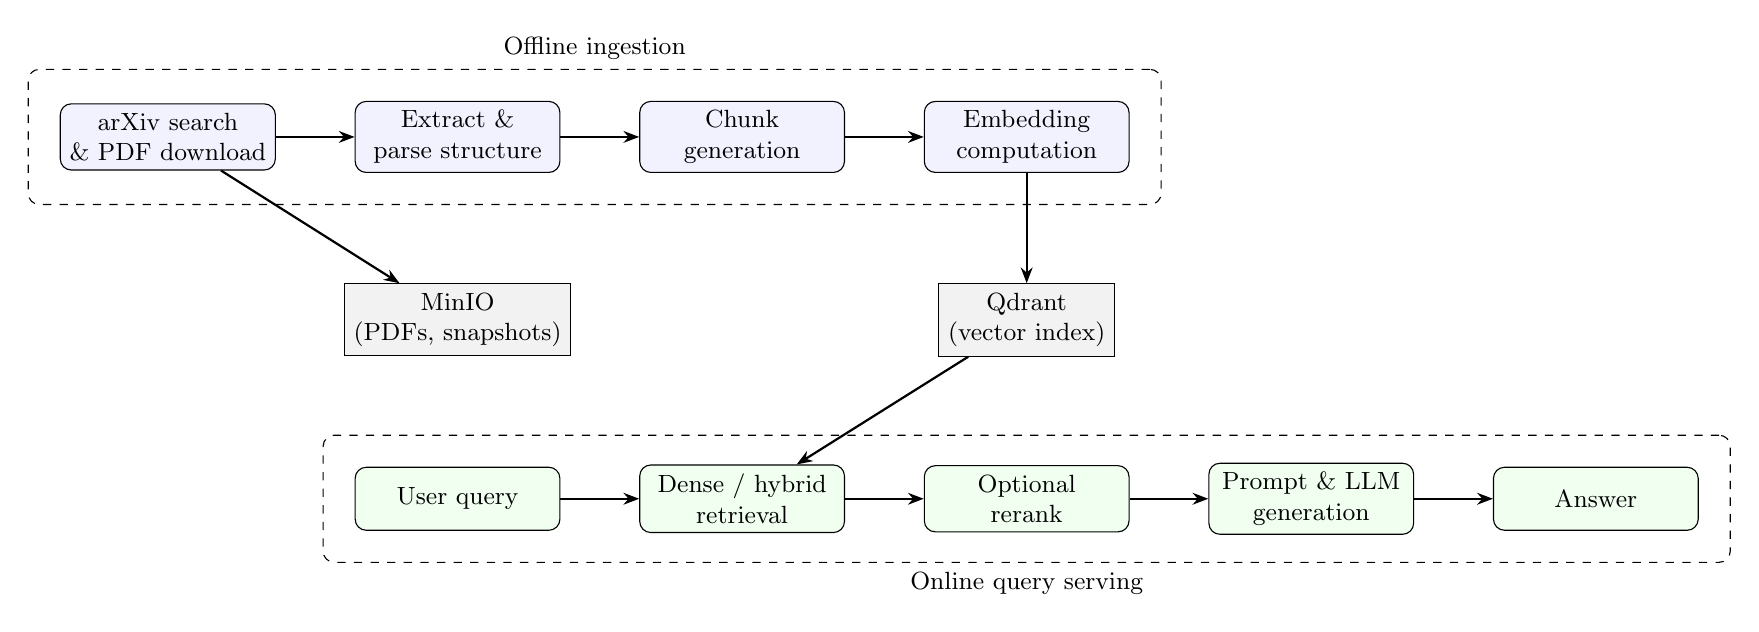
\begin{tikzpicture}[
    node distance=8mm and 10mm,
    font=\small,
    box/.style={draw, rounded corners, align=center, minimum height=8mm, minimum width=26mm, fill=blue!5},
    store/.style={draw, align=center, minimum height=8mm, minimum width=22mm, fill=gray!10},
    arr/.style={-{Stealth[length=2mm]}, thick},
]
% Ingestion row (offline)
\node[box] (search) {arXiv search\\ \& PDF download};
\node[box, right=of search] (parse) {Extract \&\\ parse structure};
\node[box, right=of parse] (chunk) {Chunk\\ generation};
\node[box, right=of chunk] (embed) {Embedding\\ computation};

% Stores
\node[store, below=14mm of parse] (minio) {MinIO\\ (PDFs, snapshots)};
\node[store, below=14mm of embed] (qdrant) {Qdrant\\ (vector index)};

% Query row (online)
\node[box, fill=green!6, below=14mm of minio] (query) {User query};
\node[box, fill=green!6, right=of query] (retrieve) {Dense / hybrid\\ retrieval};
\node[box, fill=green!6, right=of retrieve] (rerank) {Optional\\ rerank};
\node[box, fill=green!6, right=of rerank] (gen) {Prompt \& LLM\\ generation};
\node[box, fill=green!6, right=of gen] (answer) {Answer};

% Ingestion arrows
\draw[arr] (search) -- (parse);
\draw[arr] (parse) -- (chunk);
\draw[arr] (chunk) -- (embed);
\draw[arr] (search) -- (minio);
\draw[arr] (embed) -- (qdrant);

% Query arrows
\draw[arr] (query) -- (retrieve);
\draw[arr] (retrieve) -- (rerank);
\draw[arr] (rerank) -- (gen);
\draw[arr] (gen) -- (answer);
\draw[arr] (qdrant) -- (retrieve);

\begin{scope}[on background layer]
    \node[draw, dashed, rounded corners, fit=(search)(embed), inner sep=4mm, label=above:{Offline ingestion}] {};
    \node[draw, dashed, rounded corners, fit=(query)(answer), inner sep=4mm, label=below:{Online query serving}] {};
\end{scope}
\end{tikzpicture}%
}
\caption{ArxivRAG pipeline. Offline ingestion (top) builds the corpus and vector index; online query serving (bottom) retrieves, optionally reranks, and generates grounded answers. MinIO and Qdrant persist artifacts across both phases.}
\label{fig:pipeline}
\end{figure}

The design deliberately decouples indexing, retrieval, and generation, so that each stage can be configured and evaluated independently — a property exploited by the staged benchmark of Chapter~5 and by the interactive application of Chapter~7, which reuses the same stages under live serving defaults.

\section{Infrastructure and Components}
\begin{itemize}
    \item \textbf{Storage:} MinIO for documents and frozen corpus snapshots.
    \item \textbf{Vector DB:} Qdrant for embedding search.
    \item \textbf{Embedding model:} \texttt{google/embeddinggemma-300m}, from Google's Gemma family \cite{gemmateam2024gemma}.
    \item \textbf{Reranker:} \texttt{cross-encoder/ms-marco-MiniLM-L-6-v2} (optional) \cite{nogueira2019bert}.
    \item \textbf{Generator:} DeepSeek-V3 (\texttt{deepseek-chat}) through an OpenAI-compatible client \cite{deepseek2024v3}.
\end{itemize}
Splitting these components lets indexing, retrieval, and generation settings be controlled independently during experiments.

\section{Corpus Construction and Chunking}
For each query topic the system searches arXiv, filters candidate papers by abstract similarity (retaining the top $6$), and downloads their PDFs. Text is extracted and parsed into a section hierarchy, then segmented into chunks. Chunking is treated as a first-class modeling decision; the strongest strategies studied are:
\begin{itemize}
    \item \textbf{Structure-Aware Overlap:} hierarchy-aware chunking over parsed sections with a target of $650$ tokens (maximum $900$) and an overlap ratio of $0.12$ (roughly a $78$-token carryover); abstract and conclusion blocks are preserved as standalone chunks.
    \item \textbf{Semantic Paragraph Grouping:} paragraph-level grouping by adjacent-embedding similarity (threshold $0.75$) capped at $900$ tokens, falling back to structure-aware behavior when embeddings are unavailable.
\end{itemize}
Chunk embeddings are stored in Qdrant, keyed with paper and section metadata that is later reused for both relevance judgments and prompt provenance.

\section{Retrieval Modes}
Two retrieval paths are available over the chunk index:
\begin{itemize}
    \item \textbf{Dense retrieval} by cosine similarity over embedding vectors. The dense path supports Maximal Marginal Relevance (MMR, $\lambda=0.7$) for diversity-aware selection, balancing query relevance against redundancy among selected chunks \cite{carbonell1998mmr}.
    \item \textbf{Hybrid retrieval} combining dense and BM25 signals \cite{robertson2009bm25}, fused with equal weights ($0.5/0.5$) after min--max normalization of each score distribution so that the two heterogeneous scales are comparable.
\end{itemize}

\section{Reranking}
An optional cross-encoder reranking stage can reorder a candidate pool before the final top-$k$ chunks are selected \cite{nogueira2019bert}. The pool size is derived from the requested cut-off as $\operatorname{clip}(4k,\,16,\,64)$ candidates: it scales with $k$ but is bounded to keep cross-encoder scoring — which is far more expensive than a bi-encoder — within a fixed latency budget. Unlike the bi-encoder retriever, the cross-encoder jointly encodes the query and each candidate, yielding sharper relevance estimates at higher per-candidate cost.

\section{Prompt Engineering}
Prompt design is intentionally constrained to reduce stylistic hedging and enforce grounded, technical answers. The system message instructs the model to answer directly, to avoid filler phrases such as ``Based on the provided context,'' and to rely only on the supplied retrieved passages. The user prompt then injects the retrieved chunks together with explicit source metadata (paper title, arXiv identifier, section label) followed by the question. Surfacing provenance keeps generation consistent across retrieval configurations and makes it possible to trace each answer back to its supporting evidence.

\section{Generation and Context Budgeting}
Generation uses DeepSeek-V3 through an OpenAI-compatible client with \texttt{temperature}${=}0.7$, \texttt{max\_tokens}${=}2048$, and a configured context window of $8192$ tokens \cite{deepseek2024v3}. Because retrieved context can exceed this window, the system budgets context heuristically before prompting: it allocates a token-aware character budget per chunk, truncates over-long chunks, and retries with fewer chunks if the assembled prompt still exceeds the context limit. This keeps the pipeline robust to variable retrieval depth while preserving the highest-ranked evidence.

\chapter{Evaluation Methodology}

\section{Benchmark Dataset}
The practical evaluation used a manually curated benchmark of 49 examples. Each record includes:
\begin{itemize}
    \item a unique ID,
    \item topic keywords,
    \item a natural-language question,
    \item gold passages for relevance supervision.
\end{itemize}

\section{Reproducibility Setup}
Because arXiv content evolves, corpus snapshots were frozen per topic. This ensured all experiments compared settings on the same document set.

\section{Metrics}
Retrieval quality is measured with five metrics, all reported at the retrieval cut-off $k$:
\begin{itemize}
    \item \textbf{Hit@k} (Success@k): $1$ if at least one relevant chunk appears in the top-$k$, else $0$. This corresponds to the metric labelled ``Recall@k'' in the practical report.
    \item \textbf{Coverage@k}: paper-level coverage, $|\text{retrieved paper IDs}_k \cap \text{gold paper IDs}| / |\text{gold paper IDs}|$. Because each chunk belongs to one paper, this is structurally capped at $\min(k,|\text{gold}|)/|\text{gold}|$ and is therefore most meaningful at $k \geq |\text{gold}|$.
    \item \textbf{Precision@k}: fraction of the top-$k$ chunks that are relevant.
    \item \textbf{Mean Reciprocal Rank (MRR)}: reciprocal rank of the first relevant chunk.
    \item \textbf{Mean Average Precision (MAP)}: mean over queries of Average Precision, rewarding relevant chunks ranked early.
\end{itemize}

Relevance is graded: a chunk scores $1.0$ if its paper ID is a gold document, otherwise the maximum cosine similarity between the chunk and any gold passage (clipped to $[0,1]$); a chunk counts as relevant for the binary metrics when this grade meets a fixed threshold. Crucially, relevance is scored by a \emph{fixed judge embedder} that is held constant across all experiments, so that relevance labels do not drift when the retrieval embedding model is varied (Section~\ref{sec:phase3}).

\section{Experimental Design}
Three phases were used:
\begin{itemize}
    \item \textbf{Phase 1:} compare chunking strategies under fixed retrieval settings (dense, top-$k=8$, no reranking).
    \item \textbf{Phase 2:} sweep top-$k \in \{3,5,10\}$, retrieval mode (dense/hybrid), and reranking (on/off) using the best chunker.
    \item \textbf{Phase 3:} hold the winning chunker and best retrieval configuration fixed and compare embedding models, scoring all of them against the same fixed judge embedder.
\end{itemize}

\section{Statistical Analysis}
All configurations are evaluated on the same 49 queries, enabling paired comparisons. For every metric we report the mean and a 95\% bootstrap confidence interval over queries. Selected pre-registered comparisons are tested with a two-sided paired bootstrap and a Wilcoxon signed-rank test. All randomness is seeded for reproducibility.

\chapter{Results and Discussion}

\section{Phase 1: Chunking Strategy}
Table~\ref{tab:phase1} compares the four chunking strategies under fixed dense retrieval. Fixed-window overlap is strongest on every metric, and is selected as the winning chunker for the subsequent phases. Semantic paragraph grouping is clearly weakest, indicating that similarity-based paragraph merging fragments evidence in a way that hurts retrieval on this corpus.

\begin{table}[htbp]
\centering
\caption{Phase 1: chunking-strategy comparison (dense, top-$k=8$, no rerank).}
\label{tab:phase1}
\begin{tabular}{lccccc}
\toprule
Chunking strategy & Hit@k & Coverage@k & P@k & MRR & MAP \\
\midrule
\texttt{STRUCTURE\_AWARE\_OVERLAP} & 0.8776 & 0.3279 & 0.3061 & 0.6511 & 0.5384 \\
\texttt{SEMANTIC\_PARAGRAPH\_GROUPING} & 0.6531 & 0.1374 & 0.1556 & 0.3546 & 0.3419 \\
\texttt{FIXED\_WINDOW\_OVERLAP} & \textbf{0.9388} & \textbf{0.4925} & \textbf{0.4362} & \textbf{0.7475} & \textbf{0.6480} \\
\texttt{SECTION\_LEVEL\_CHUNKING} & 0.9184 & 0.3714 & 0.3444 & 0.5931 & 0.5212 \\
\bottomrule
\end{tabular}
\end{table}

\section{Phase 2: Retrieval Configuration}
Table~\ref{tab:phase2} sweeps top-$k$, retrieval mode, and reranking on the winning chunker. Dense retrieval at top-$k=10$ without reranking gives the best coverage (Coverage@k $=0.5204$), Hit@k ($0.9592$), and MRR ($0.7495$). Reranking raises Precision@k at small $k$ (e.g.\ P@3 $=0.5918$ with dense$+$rerank) but lowers coverage, confirming it as a precision-oriented option rather than a coverage-oriented one.

\begin{table}[htbp]
\centering
\caption{Phase 2: retrieval-configuration sweep on the winning chunker.}
\label{tab:phase2}
\begin{tabular}{lccccccc}
\toprule
top-$k$ & Retrieval & Rerank & Hit@k & Coverage@k & P@k & MRR & MAP \\
\midrule
3 & dense & no & 0.8571 & 0.2537 & 0.5170 & 0.7313 & \textbf{0.7126} \\
3 & dense & yes & 0.7959 & 0.2088 & \textbf{0.5918} & 0.7279 & 0.7092 \\
3 & hybrid & no & 0.7551 & 0.1952 & 0.5374 & 0.6293 & 0.6224 \\
3 & hybrid & yes & 0.7755 & 0.1946 & 0.5578 & 0.6837 & 0.6650 \\
5 & dense & no & 0.9184 & 0.3694 & 0.4857 & 0.7446 & 0.6814 \\
5 & dense & yes & 0.8571 & 0.2776 & 0.5429 & 0.7150 & 0.6809 \\
5 & hybrid & no & 0.7755 & 0.2327 & 0.5265 & 0.6333 & 0.6169 \\
5 & hybrid & yes & 0.8367 & 0.2694 & 0.5224 & 0.6963 & 0.6461 \\
10 & dense & no & \textbf{0.9592} & \textbf{0.5204} & 0.4020 & \textbf{0.7495} & 0.6400 \\
10 & dense & yes & 0.9388 & 0.3810 & 0.5306 & 0.7226 & 0.6500 \\
10 & hybrid & no & 0.8980 & 0.3381 & 0.5082 & 0.6523 & 0.6170 \\
10 & hybrid & yes & 0.9388 & 0.3830 & 0.5041 & 0.7084 & 0.6285 \\
\bottomrule
\end{tabular}
\end{table}

\section{Phase 3: Embedding-Model Comparison}
\label{sec:phase3}
Table~\ref{tab:phase3} compares three embedding models under the winning chunker and best retrieval configuration, with relevance scored by a single fixed judge embedder so that the labels are identical across models. The baseline \texttt{embeddinggemma-300m} is best or tied on all metrics, but the margins are small. Notably, the much smaller \texttt{bge-small-en-v1.5} (384-dim) matches the baseline on Hit@k and Coverage@k, suggesting that embedding size is not the dominant factor on this benchmark. These models were run without model-specific query/passage prompt templates, so the results for the \texttt{bge} family should be read as a lower bound.

\begin{table}[htbp]
\centering
\caption{Phase 3: embedding-model comparison (fixed window overlap, dense, top-$k=10$, no rerank; fixed judge embedder).}
\label{tab:phase3}
\begin{tabular}{lcccccc}
\toprule
Embedding model & dim & Hit@k & Coverage@k & P@k & MRR & MAP \\
\midrule
\texttt{google/embeddinggemma-300m} & 768 & \textbf{0.9592} & \textbf{0.5204} & 0.4020 & \textbf{0.7495} & \textbf{0.6400} \\
\texttt{BAAI/bge-small-en-v1.5} & 384 & \textbf{0.9592} & 0.5027 & 0.4020 & 0.7340 & 0.5935 \\
\texttt{BAAI/bge-base-en-v1.5} & 768 & 0.9388 & 0.4782 & \textbf{0.4102} & 0.6932 & 0.6116 \\
\bottomrule
\end{tabular}
\end{table}

\section{Statistical Significance}
Table~\ref{tab:significance} reports paired tests for the main comparisons. On Hit@k, none of the differences reach significance at $\alpha=0.05$: Hit@k saturates near $0.9$ on this corpus, so it has little power to separate configurations (a ceiling effect). The more granular Coverage@k and MAP are more discriminative, and comparative claims below rest on them rather than on Hit@k.

\begin{table}[htbp]
\centering
\caption{Paired significance tests (49 queries, seed 42). $\Delta$ is the paired mean difference; bold $p<0.05$.}
\label{tab:significance}
\begin{tabular}{lcccc}
\toprule
Comparison (metric) & $\Delta$ & 95\% CI & boot $p$ & Wilcoxon $p$ \\
\midrule
Ph2: best vs.\ 2nd-best (Hit@k) & +0.0204 & [+0.0000, +0.0612] & 0.6293 & 0.3173 \\
Ph2: dense vs.\ hybrid ($k{=}10$) (Hit@k) & +0.0612 & [+0.0000, +0.1429] & 0.1200 & 0.0833 \\
Ph3: gemma vs.\ \texttt{bge-small-en-v1.5} (Hit@k) & +0.0000 & [+0.0000, +0.0000] & 1.0000 & 1.0000 \\
Ph3: gemma vs.\ \texttt{bge-small-en-v1.5} (MAP) & +0.0464 & [-0.0279, +0.1213] & 0.2164 & 0.2852 \\
Ph3: gemma vs.\ \texttt{bge-base-en-v1.5} (Hit@k) & +0.0204 & [+0.0000, +0.0612] & 0.6228 & 0.3173 \\
Ph3: gemma vs.\ \texttt{bge-base-en-v1.5} (MAP) & +0.0284 & [-0.0420, +0.0981] & 0.4252 & 0.2935 \\
\bottomrule
\end{tabular}
\end{table}

\section{Interpretation}
Chunking is the largest single design variable: the gap between the best and worst chunker (Table~\ref{tab:phase1}) dwarfs the effect of retrieval mode, reranking, or embedding model. Dense retrieval consistently matches or beats hybrid retrieval on this corpus, and the practical default of fixed-window chunking with dense retrieval at top-$k=10$ and no reranking remains the best all-round operating point. The embedding-model comparison shows that, once chunking and retrieval are fixed, the choice of embedding model has only a small (and here non-significant) effect. Taken together with the significance analysis, the honest reading is that the strongest \emph{observed} configuration is a reasonable default, but several alternatives are statistically indistinguishable given the benchmark size. Chapter~7 discusses how these findings relate to the interactive application's current serving defaults, which still expose all four chunkers rather than locking to the Phase~2 winner.

\section{Limitations}
\begin{itemize}
    \item Small benchmark size (49 queries), which limits statistical power, as the significance tests make explicit.
    \item Hit@k saturates on this corpus and is therefore weakly discriminative; Coverage@k is capped at low $k$; both caveats are addressed by leaning on MAP.
    \item Embedding models were compared without model-specific prompt templates.
    \item Relevance grading uses a fixed embedding-based judge, which anchors labels but is itself an automatic proxy for human relevance judgements.
    \item Retrieval-only evaluation: generated-answer quality is not scored.
\end{itemize}

\chapter{Application Architecture}

The evaluation in Chapters~5 and~6 treats ArxivRAG as a retrieval experiment: a frozen corpus, a fixed query set, and rank-aware metrics. That is the right setting for comparing design choices, but it is not how a scientific QA system is used. This chapter documents the interactive application that wraps the pipeline of Chapter~4 in a working user-facing stack. The aim is not a full software-engineering specification; it is to show how the measured pipeline is served, where serving defaults still differ from the empirically strongest configuration, and which application-level decisions --- provenance, ephemeral indexing, multi-strategy comparison --- are part of the RAG contract rather than incidental UI.

\section{Two Instantiations of One Pipeline}

The codebase maintains two instantiations of the same core modules (arXiv retrieval, PDF parsing, chunking, embedding, Qdrant indexing, and optional hybrid/rerank retrieval):

\begin{itemize}
    \item \textbf{Evaluation harness.} CLI scripts freeze a corpus snapshot into a dedicated MinIO bucket, re-index it under a chosen configuration, and score retrieval without calling the generator. This path is deterministic by design (Chapter~5).
    \item \textbf{Interactive application.} A FastAPI service and a Next.js client fetch papers live from arXiv, index them into a separate storage namespace, generate grounded answers, and return cited sources. The index is rebuilt per query and discarded afterwards.
\end{itemize}

Sharing the pipeline code keeps the two paths comparable: a chunking strategy or retrieval constant changed in one place is the one the other path will use. Separating storage namespaces (\texttt{eval-frozen-corpus} versus \texttt{interactive-rag-pdfs}) prevents a live query from contaminating a frozen benchmark, and vice versa.

\section{Layered Stack}

The application is a three-tier local stack, shown in Figure~\ref{fig:app-architecture}. Infrastructure is the same Docker Compose pair already used for evaluation (MinIO for PDFs, Qdrant for vectors and paper metadata). The application adds a generation client and a browser interface on top.

\begin{figure}[htbp]
\centering
\resizebox{\textwidth}{!}{%
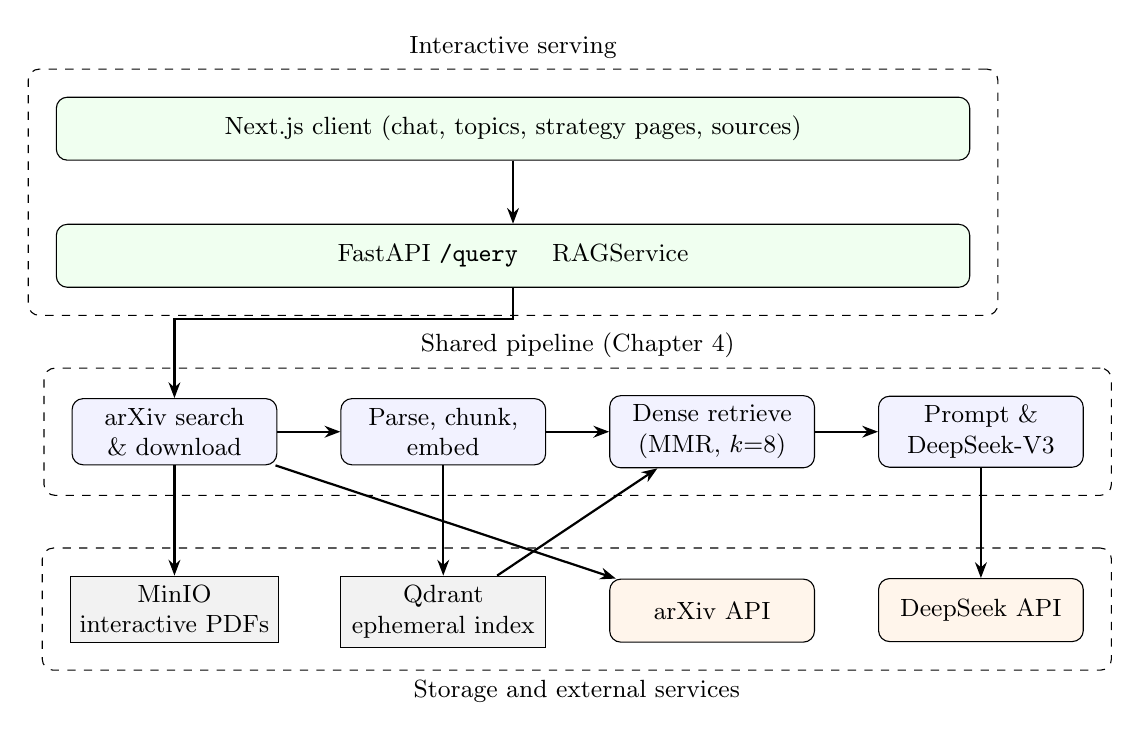
\begin{tikzpicture}[
    node distance=8mm and 8mm,
    font=\small,
    box/.style={draw, rounded corners, align=center, minimum height=8mm, minimum width=26mm, fill=blue!5},
    store/.style={draw, align=center, minimum height=8mm, minimum width=26mm, fill=gray!10},
    ext/.style={draw, rounded corners, align=center, minimum height=8mm, minimum width=26mm, fill=orange!8},
    arr/.style={-{Stealth[length=2mm]}, thick},
]
\node[box, fill=green!6, minimum width=116mm] (ui) {Next.js client (chat, topics, strategy pages, sources)};
\node[box, fill=green!6, below=of ui, minimum width=116mm] (api) {FastAPI \texttt{/query} \quad RAGService};

\node[box, below=14mm of api.south west, anchor=north west, xshift=2mm] (arxiv) {arXiv search\\ \& download};
\node[box, right=of arxiv] (chunk) {Parse, chunk,\\ embed};
\node[box, right=of chunk] (ret) {Dense retrieve\\ (MMR, $k{=}8$)};
\node[box, right=of ret] (llm) {Prompt \&\\ DeepSeek-V3};

\node[store, below=14mm of arxiv] (minio) {MinIO\\ interactive PDFs};
\node[store, below=14mm of chunk] (qdrant) {Qdrant\\ ephemeral index};
\node[ext, below=14mm of ret] (ax) {arXiv API};
\node[ext, below=14mm of llm] (ds) {DeepSeek API};

\draw[arr] (ui) -- (api);
\draw[arr] (api.south) -- ++(0,-4mm) -| (arxiv.north);
\draw[arr] (arxiv) -- (chunk);
\draw[arr] (chunk) -- (ret);
\draw[arr] (ret) -- (llm);
\draw[arr] (arxiv) -- (minio);
\draw[arr] (chunk) -- (qdrant);
\draw[arr] (qdrant) -- (ret);
\draw[arr] (arxiv) -- (ax);
\draw[arr] (llm) -- (ds);

\begin{scope}[on background layer]
    \node[draw, dashed, rounded corners, fit=(ui)(api), inner sep=3.5mm, label=above:{Interactive serving}] {};
    \node[draw, dashed, rounded corners, fit=(arxiv)(llm), inner sep=3.5mm, label=above:{Shared pipeline (Chapter~4)}] {};
    \node[draw, dashed, rounded corners, fit=(minio)(ds), inner sep=3.5mm, label=below:{Storage and external services}] {};
\end{scope}
\end{tikzpicture}%
}
\caption{Interactive ArxivRAG application. The Next.js client calls a FastAPI service that orchestrates live arXiv retrieval, ephemeral indexing, and grounded generation. MinIO and Qdrant are the same infrastructure as in the evaluation path, under a separate namespace.}
\label{fig:app-architecture}
\end{figure}

\paragraph{Presentation.} The client is a Next.js (React) single-page chat interface. The user supplies two fields that match the evaluation record schema: comma-separated \emph{topics} for arXiv keyword search, and a natural-language \emph{question} for embedding and retrieval. Assistant messages render markdown, list cited papers with arXiv links, and paginate across the four chunking strategies so that answers can be compared side by side. A session can be exported as a self-contained HTML transcript.

\paragraph{Application.} FastAPI exposes \texttt{POST /query} and \texttt{GET /health}. On startup it initializes storage, the embedding model, the Qdrant collection, the arXiv retriever, and the DeepSeek client; on shutdown it clears the interactive index. The blocking pipeline runs in a worker thread so that the event loop is not stalled for the duration of search, download, and embedding. CORS is restricted to the local frontend origin.

\paragraph{Shared pipeline and infrastructure.} Paper discovery, PDF extraction with PyMuPDF, the four chunkers, EmbeddingGemma, and Qdrant indexing are the components of Chapter~4. Generation uses DeepSeek-V3 (\texttt{deepseek-chat}) through an OpenAI-compatible client, with the same prompt template and context-budgeting heuristics already described there.

\section{Query Lifecycle}

A single \texttt{/query} request is a complete retrieve-then-read pass over a freshly built, query-specific corpus:

\begin{enumerate}
    \item Topics are converted to an arXiv search string (multi-word terms quoted as phrases) and up to 20 papers are retrieved.
    \item Abstracts are embedded and ranked by cosine similarity to the question; the top 6 papers are downloaded.
    \item The interactive Qdrant collection and MinIO objects are cleared, then each PDF is parsed, chunked under \emph{all four} strategies, embedded, and stored, with abstracts kept as standalone chunks.
    \item For each strategy, dense retrieval with Maximal Marginal Relevance ($\lambda=0.7$) returns $k=8$ chunks, expanded to neighbouring chunk positions, and DeepSeek generates an answer from those passages plus source metadata.
    \item The response is a list of four results, each with the strategy identity, the generated answer, and the unique papers cited from the retrieved chunks.
\end{enumerate}

The ephemeral index is a deliberate product decision, not an accident of prototyping. Live arXiv search is non-stationary: a query about ``agentic RAG'' today will not retrieve the same papers as the same query next month. Rebuilding the index per request keeps answers aligned with the papers just fetched, at the cost of latency (search, download, parse, and four-way embedding all sit on the critical path). The evaluation path pays that cost once, when the corpus is frozen.

\section{Provenance and Multi-Strategy Comparison}

Two application-level choices are worth stating as RAG design, not as frontend polish.

\paragraph{Provenance.} Each retrieved chunk is injected into the prompt with paper title, arXiv identifier, and section label. The API then extracts unique papers from the chunks actually sent to the generator and returns them as sources. The UI renders those sources as outbound links to \texttt{arxiv.org/abs/...}. This closes the loop that the RAG framework motivates \cite{lewis2020rag} --- generation grounded in non-parametric memory --- with an inspectable paper trail, which is especially important in a scientific setting where a fluent answer without a citable source is of limited use.

\paragraph{Four answers per query.} The application does not hide chunking behind a single default. It indexes and answers under every strategy and lets the user page through the four outputs. That choice has a research reading: Chapter~6 found chunking to be the dominant design variable, with a large gap between the best and worst strategy. Serving all four is a qualitative counterpart to Table~\ref{tab:phase1}. It also has an engineering cost: four indexes and four generations per query. A production deployment that had already committed to a winner would not pay that cost.

\section{Serving Defaults versus Experimental Findings}

The evaluation identified a practical operating point: fixed-window overlap, dense retrieval, top-$k=10$, reranking off. The interactive path currently uses dense retrieval at $k=8$ with MMR and neighbour expansion, and it generates under all four chunkers rather than under the winning one. Hybrid retrieval and cross-encoder reranking are implemented in the shared retrieval module and were swept in Phase~2, but they are not enabled on the live path.

This gap is honest rather than accidental. The application is still a developmental system whose UI is designed to \emph{inspect} chunking, not to lock a production default. The topics/question split, the embedding model, the generator, and the prompt template are already aligned with the pipeline that was measured. What is not yet aligned is the serving configuration itself: adopting the Phase~2 winner as the default answer, and keeping the four-strategy view as an optional comparison mode, is the natural next engineering step. Until generated-answer quality is scored, that step remains a retrieval-informed heuristic rather than a generation-validated one.

\section{Limitations of the Deployed Application}

The application demonstrates that the pipeline is usable, not that it is production-ready.

\begin{itemize}
    \item \textbf{Latency.} Per-query search, download, and four-way indexing make response time dominated by corpus construction rather than by nearest-neighbour search.
    \item \textbf{No persistence.} Papers and embeddings are discarded after each request, so repeated questions re-pay the same cost and cannot accumulate a user-specific library.
    \item \textbf{Live, non-reproducible corpora.} Unlike the frozen evaluation snapshots, two identical queries can retrieve different papers as arXiv changes.
    \item \textbf{Single-user local deployment.} The stack is designed for a researcher running Docker, the API, and the frontend on one machine; it is not a multi-tenant service.
    \item \textbf{Ungraded generation.} The application produces answers and citations, but this thesis does not score faithfulness or answer correctness --- the same out-of-scope boundary stated in Chapter~1.
\end{itemize}

These limitations are the bridge into future work: a persistent index, a serving configuration that follows the evaluation winner, and a generation-quality evaluation that can be run against the same \texttt{/query} path the UI already uses.

\chapter{Future Work}

The extended evaluation in this thesis realised two extensions that were previously only planned: additional rank-aware IR metrics (MAP alongside Hit@k, Coverage@k, Precision@k, and MRR) and an embedding-model comparison under a fixed relevance judge, both with confidence intervals and paired significance testing. The main remaining direction is to connect retrieval quality to \emph{generation} quality: generating answers from the retrieved context and scoring them for faithfulness and answer relevance, then testing whether the best retrieval configuration is also the best generation configuration. The interactive application already produces those answers and can optionally return the retrieved chunks (\texttt{include\_debug\_context}), so it is a natural vehicle for that evaluation rather than a separate prototype.

On the application side, two engineering follow-ups follow directly from Chapter~7. First, persist papers and embeddings across queries (or cache by arXiv identifier) so that latency is not dominated by repeated download and indexing. Second, adopt the empirically strongest retrieval configuration --- fixed-window chunking, dense retrieval, top-$k=10$, no reranking --- as the default answer, keeping the four-strategy view as an optional comparison mode. Further evaluation work includes enlarging the benchmark to increase statistical power, adding model-specific prompt templates for the embedding comparison, and validating the automatic relevance judge against human judgements.

\chapter{Conclusion}

This thesis unifies prior seminar and practical work into a single narrative and extends the practical's evaluation. The theoretical chapters motivate RAG for scientific literature; the pipeline chapter documents the shared retrieve-then-read stack; the evaluation chapters present a reproducible, statistically grounded benchmark; and the application chapter shows how that stack is served to users, including provenance, ephemeral live indexing, and multi-strategy comparison. Fixed-window chunking with dense retrieval at top-$k=10$ and no reranking is confirmed as the strongest operating point, chunking is identified as the dominant design variable, and the embedding-model comparison shows only small, non-significant differences once chunking and retrieval are fixed. The interactive application does not yet lock to that operating point: it currently exposes all four chunkers as a qualitative inspection tool. The significance analysis tempers these conclusions appropriately given the benchmark size, and points to a larger benchmark, a serving configuration aligned with the evaluation winner, and generation-quality evaluation as the natural next steps.

\bibliography{references}

\end{document}
